%%%%%%%%%%%%%%%%%%%%%%%%%%%%%%%%%%%%%%%%%%%%%%%%%%%%%%%%%%%%%%%%%%%%%%%
%% Zusammenfassung und Ausblick
\section{Implementierung}
\label{sec:impl}

In diesem Kapitel werden einige Aspekte der Entwicklung aufgegriffen und im Detail ausgeführt. Der Name Implementierung bezieht sich nicht auf die Programmierung, sondern die Umsetzung von Schnittstellen und den Algorithmen hinter speziellen Problemen. So wird zum Beispiel in dem Unterkapitel \ref{sec:impl-rs} auf die Bewegung auf einer linearen Trajektorie eingegangen. Außerdem werden Probleme beschrieben und gelöst, die während der Umsetzung der Konzepte auftraten. Des Weiteren werden die genutzten Bibliotheken erwähnt und die Anbindung von ROS an die Konzepte. Den zentralen Aspekt in diesem Kapitel stellt jedoch Unterkapitel \ref{sec:impl-hop} dar. In diesem wird die Bestimmung für die Übergabeposition vorgestellt.

\subsection{Robotersteuerung - RATSYoubot \& RATSDummy \& RATSRose}
\label{sec:impl-rs}
In diesem Kapitel wird die Ansteuerung für die Roboter und deren Arme vorgestellt. Diese beruht vor allem auf der Kuka API für den Youbot. Außerdem wird die Bewegung auf einer linearen Trajektorie, sowie die einzelnen Aktionen die ein Roboter ausführen kann kurz aufgelistet und beschrieben.

\subsubsection{Ansteuerung der Aktoren}
Die Aktoren innerhalb der Roboter werden mit Hilfe von ROS Topics angesteuert. Diese werden von dem Controllernode \textit{youbot\_driver} ausgelesen und in die Steuersignale für die Motoren umgewandelt. Für die Ansteuerung des Arms existieren zwei Topics. Der \textit{velocity\_command}-Topic erwartet für jedes Gelenk eine Geschwindigkeitsangabe. Für diese Arbeit wird jedoch mit Positionsangaben gearbeitet. Der dazu gehörige Topic \textit{arm\_controller/position\_command} benötigt ein Array mit Gelenkkonfigurationen. Dafür wird die ROS-Bibliothek \textit{BRICS} genutzt. Diese beinhaltet Nachrichten für inverse Kinematiken, wie zum  Beispiel: Posen, Vektoren und Rotationen im Kartesischen Raum oder Aktoren Nachrichten, wie Gelenkeinstellung, Gelenkgeschwindigkeiten und Gelenkbeschleunigungen. Neben der Armansteuerung gibt es für die Gripper eine eigene Topic \textit{gripper\_controller/position\_command}. Dieser transportiert ebenfalls Gelenkeinstellungen. Dabei kann die Position der einzelnen Finger des Grippers angegeben werden. Die Werte entsprechen dabei der Distanz der Finger zu ihrer Basisposition. Ein Nachteil der Ansteuerung über die Topics ist das fehlende Feedback. Der Absender erfährt nicht, ob das Signal angekommen ist und wann die Bewegung beendet ist. Sollen Bewegungen seriell ausgeführt werden muss der ausführende Thread blockiert werden, bis die Gelenke die Zielkonfiguration erreicht haben.  Ein paralleler Thread liest die aktuelle Gelenkkonfiguration aus und berechnet eine Differenz für jedes einzelne Gelenk und die Quadratsumme über alle Gelenke. Solange die Differenz für mindestens ein Gelenk oder die Summe der Quadrate ihre Schwellwerte überschreiten blockiert ein Mutex den ausführenden Thread. Ein weiteres Problem während der Implementierung stellte die Ungenauigkeit der Ansteuerung dar. Dabei kam es großen Abweichungen an einem Gelenk, wenn es eine große Winkeländerung hatte. Dieses Überschlagen lässt sich auf die Massenträgheit des Armes und dem abrupten Abbremsen der Motoren zurückführen. Dies konnte jedoch auch durch den parallelen Thread abgefangen werden. Dieser überprüft nun auch neben der Distanz zu der Zieleinstellung, die Distanz zur letzten gemessenen Gelenkeinstellung. Ist diese nahe null, also der Arm nicht mehr in Bewegung, und die Distanz zum Ziel zu groß wurde nochmal die selbe Gelenkeinstellung an den Motorencontroller geschickt.

Die Ansteuerung der mobilen Plattform wird mit einer einzelnen Topic \textit{cmd\_vel} umgesetzt. Dabei wird eine einzelne Nachricht übermittelt. Diese beinhaltet eine Twist Nachricht aus dem \textit{geometry\_msg} Paket. In dieser Nachricht kann eine lineare und eine Winkelgeschwindigkeit angegeben werden. Diese können für die einzelnen Achsen zerlegt werden. Für die mobile Plattform werden jedoch nur die X- und Y- Achsen der linearen, sowie die Z-Achse der Rotationsgeschwindigkeit ausgelesen und als absoluten Wert gesetzt. Der Controller rechnet anschließend die benötigten Steuersignale für die einzelnen Räder und Motoren aus.

\subsubsection{Lineare Bahnbewegung}
Die lineare Bahnbewegung wird beim Aufheben, Ablegen und während der Übergabe benötigt. Dies liegt vor allem an der Kollisionsvermeidung des Objektes mit der Umwelt. Da die inverse Kinematik die Gelenkeinstellungen und nicht die Gelenkgeschwindigkeiten berechnet ist es nicht so einfach auf einer gezielten Trajektorie entlang zufahren. Der Übergang zwischen zwei Gelenkeinstellung wird nicht genau definiert. Wie in Abbildung \ref{fig:traj} dargestellt kommt es dabei durch unterschiedliche Gelenkgeschwindigkeiten zu einem Ausschlagen des Greifers. Je größer die Distanz zwischen zwei Posen, desto größer der Ausschlag. Deshalb kann dies verhindert beziehungsweise minimiert werden, indem Zwischenposen auf der Trajektorie ermittelt werden, die nacheinander angefahren werden. Dies erfordert zwar eine häufiges Aufrufen der inversen Kinematik, dafür kann eine Trajektorie mit einem geringen Ausschlag entlang gefahren werden. Tests mit dem YouBot Armen und der inversen Kinematik ergaben eine Distanz von 5 Millimetern zwischen den Zwischenposen als optimal. Bei einer kleineren Distanz reduzierte sich die Amplitude des Ausschlages weniger als vorher und steigert die Kosten durch einen häufigeren Aufruf der inversen Kinematik. Bei der Implementierung nutzt dafür vor allem die Orocos KDL Api, die auch bei der Implementierung der inversen Kinematik genutzt wird. Diese ermöglicht das Rechnen mit geometrischen Primitiven, so wurde der \lstinline|KDL::Frame| für die Abbildung von Koordinatensystemen und Posen genutzt. Dieser ermöglicht unter anderem die Bestimmung der Zwischenposen.

\begin{figure}[h]
	\centering
	\subfigure[]{%
		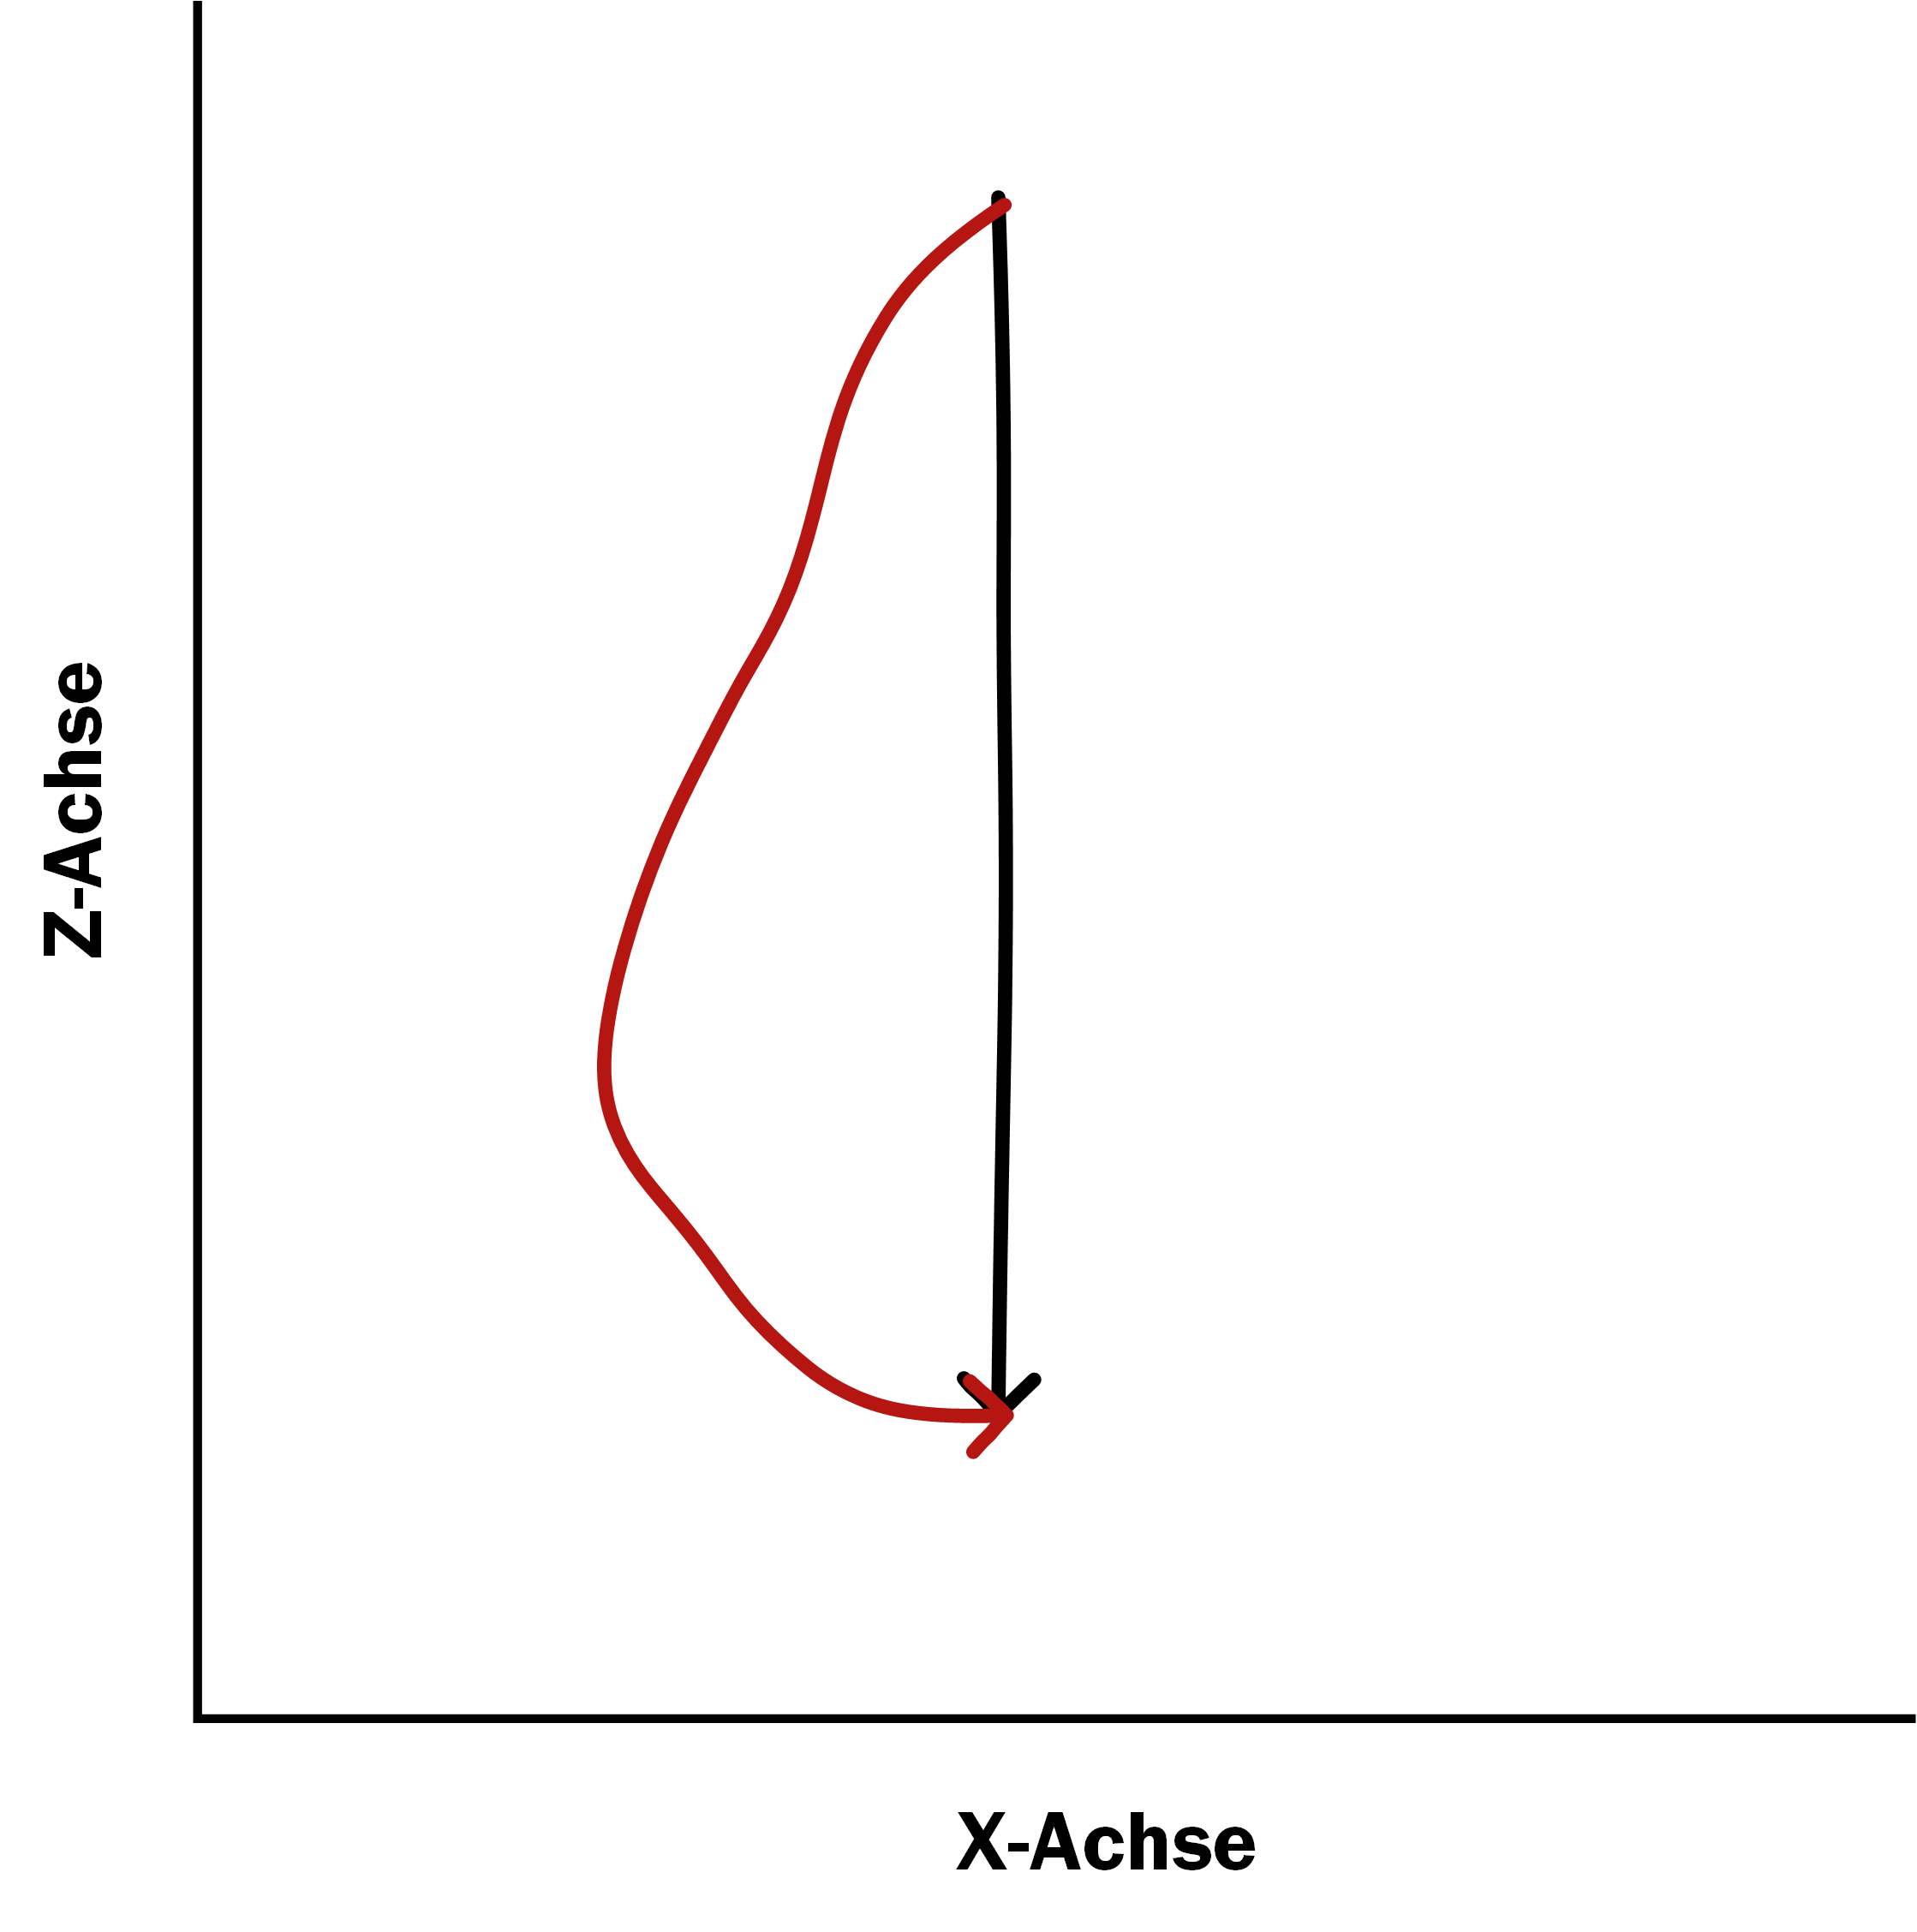
\includegraphics[scale=0.7]{fig/traj1}}
	\hfill
	\subfigure[]{%
		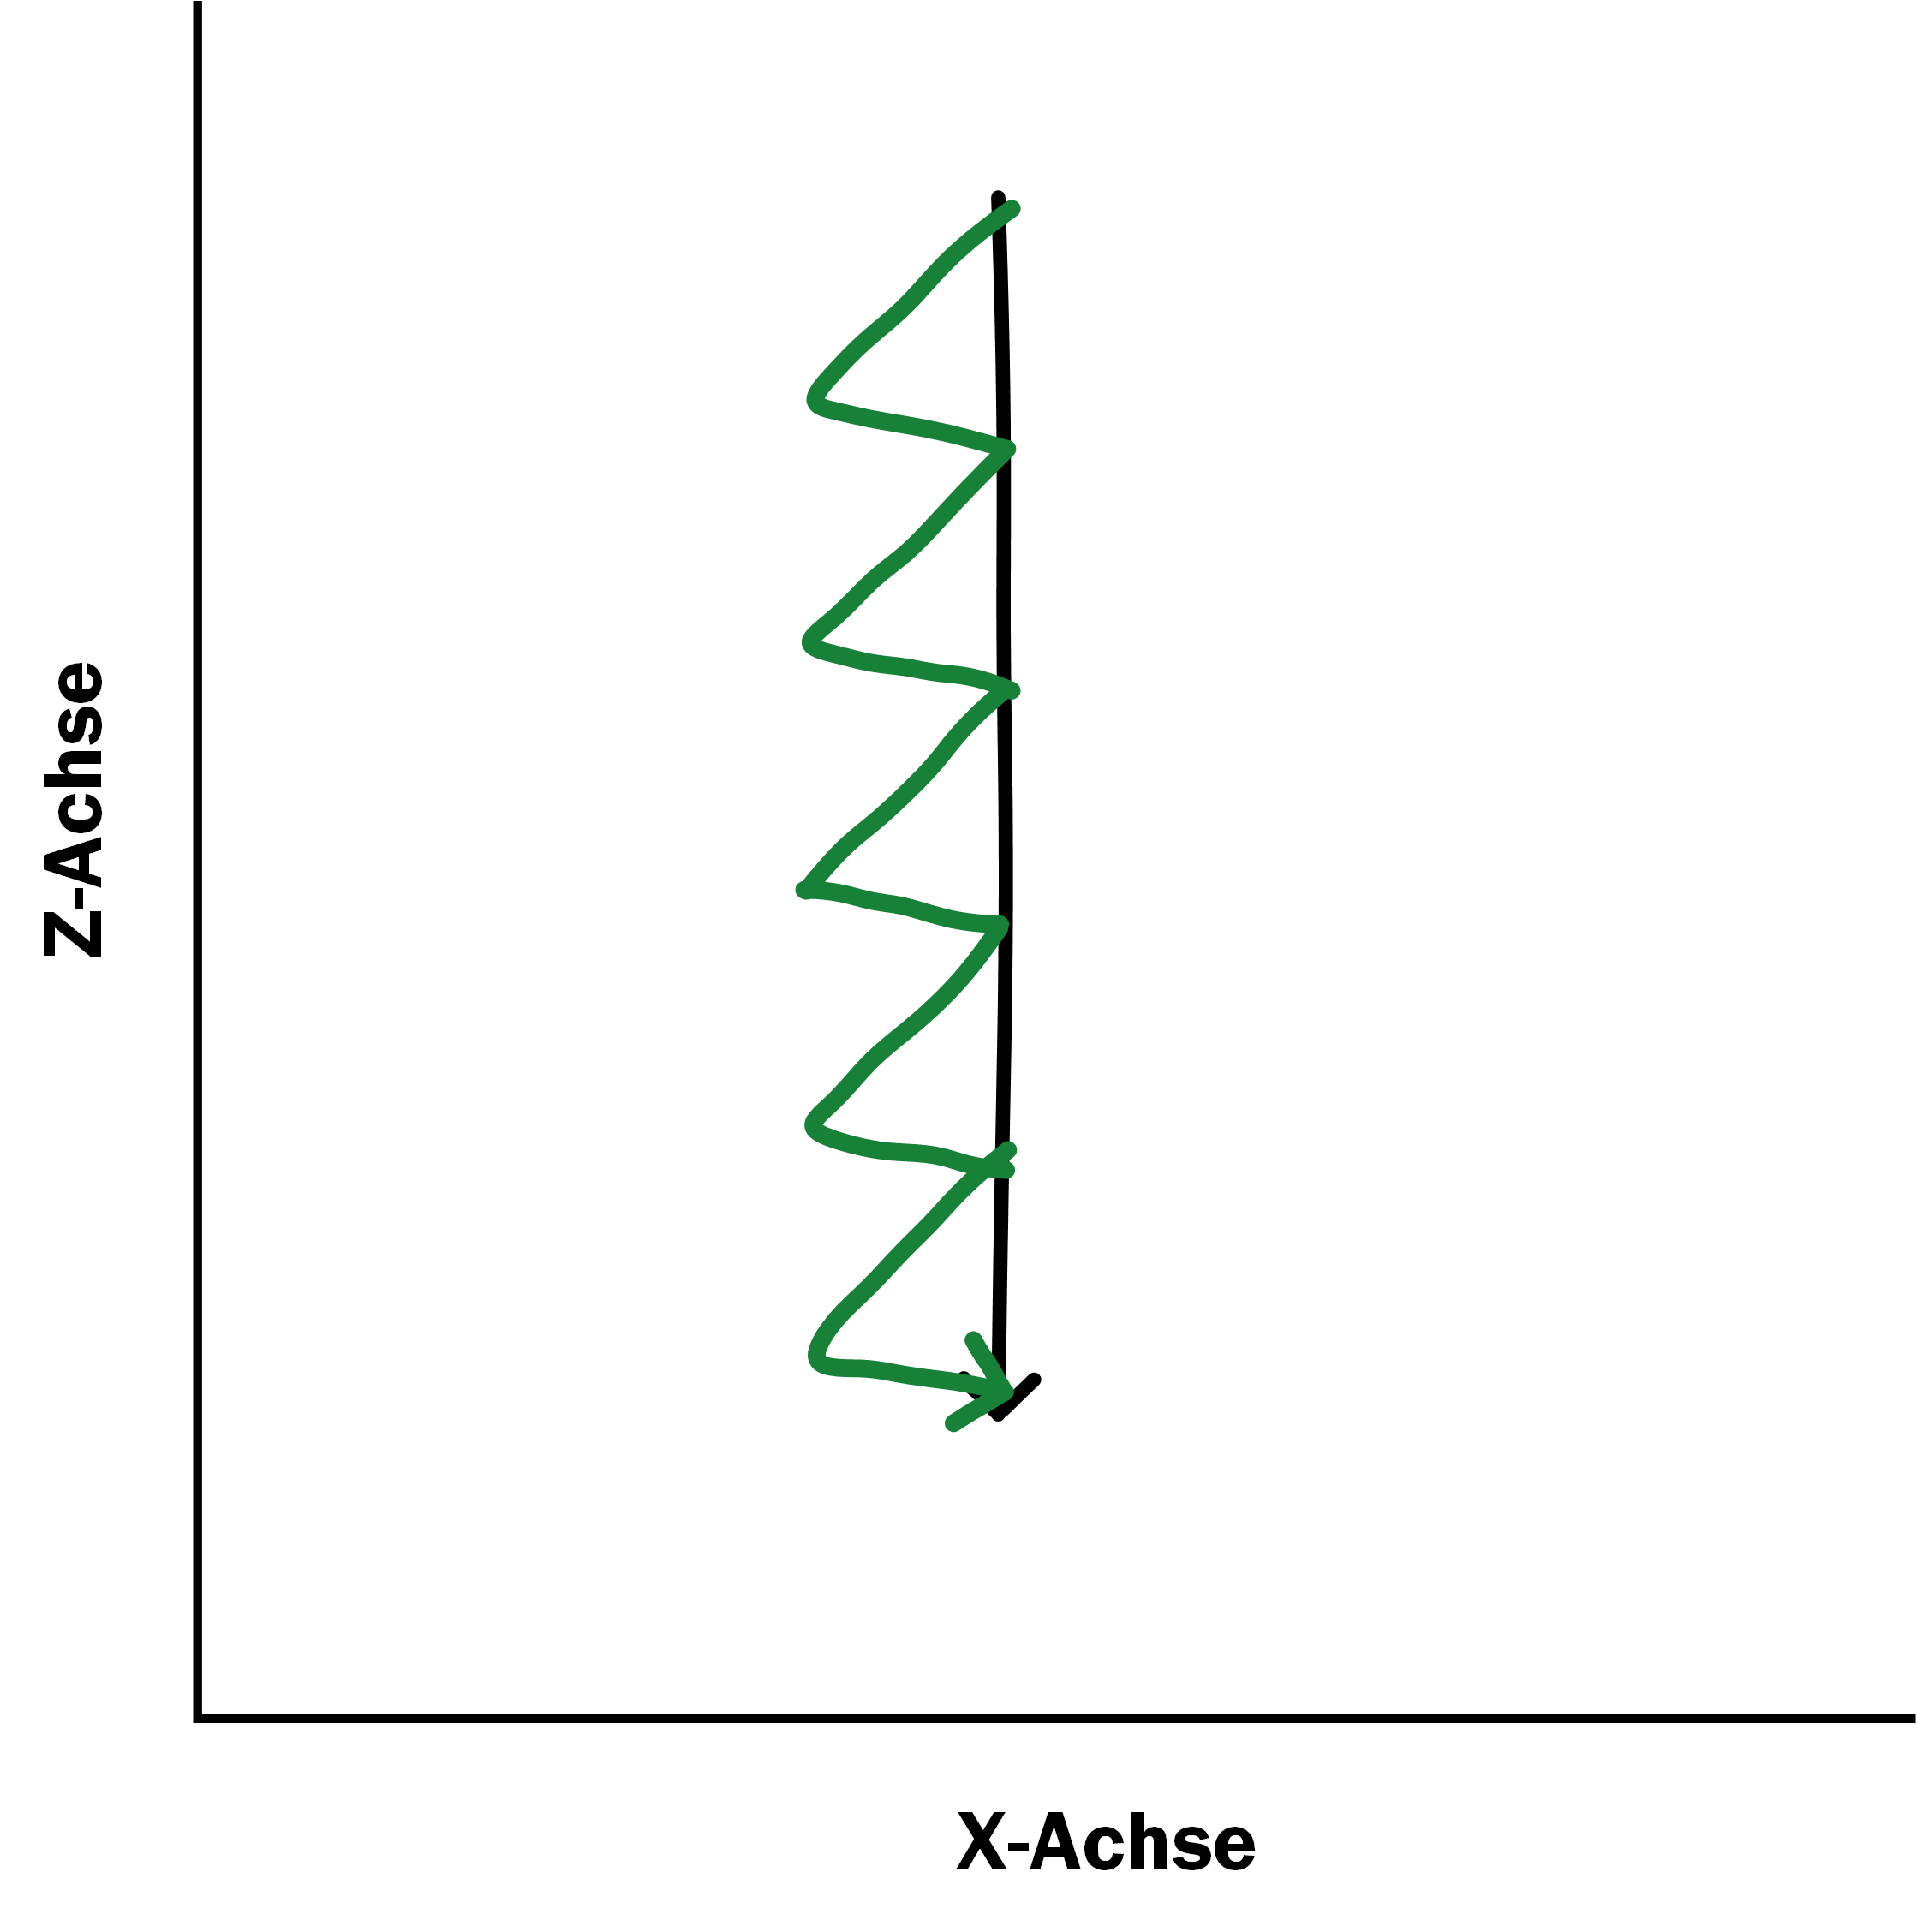
\includegraphics[scale=0.7]{fig/traj2}}
	\caption[Trajektorien des Greifers]{Die dargestellten Graphen stellen die gewünschte Trajektorie (schwarz) und die realen Trajektorien des Greifers dar. Dabei handelt es sich um eine lineare Absenkung auf der Z-Achse. Links: Trajektorie (rot) bei Angabe der Zielpose. Rechts: Trajektorie (grün) bei Angabe von Zwischenposen auf der gewünschten Trajektorie. Bildquelle: \cite{muggler2013torque}}	
	\label{fig:traj}
\end{figure}

\subsection{Raumüberwachung - RATSHawk}
\subsection{Nahfelderkennung - RATSEye}
\subsection{Koordinierung - RATSCore \& RATSMember}
\subsection{Lokale Positionierung}
\subsection{Handoverpoint}
\label{sec:impl-hop}
